%%%%%%%%%%%%%%%%%%%%%%%%%%%%%%%%%%%%%%%%%%%%%%%%%%%%%%%%%%%%%%%%%%%%%%%%
% Preamble
%%%%%%%%%%%%%%%%%%%%%%%%%%%%%%%%%%%%%%%%%%%%%%%%%%%%%%%%%%%%%%%%%%%%%%%%
\documentclass[11pt]{article}
%
% Packages and other includes
% Pagination
\usepackage[letterpaper, margin=1in]{geometry}
%
% Graphics, floats, tables
\usepackage{graphicx, color, float, array}
\graphicspath{{image/}}
%
% Fonts
\usepackage[T1]{fontenc} % best for Western European languages
\usepackage{lmodern} % Latin Modern instead of CM
\usepackage{textcomp} % required to get special symbols
%
% Math
\usepackage{amsmath, amssymb}
\usepackage{enumerate}
\usepackage{braket}
% 
% Hyperlinks
\usepackage[colorlinks,linkcolor={red},citecolor={blue},
urlcolor={blue}]{hyperref} 
%
% Definitions and settings
% Paragraph indent and spacing
\setlength{\parskip}{0.4\baselineskip}
\setlength{\parindent}{0in}
%
% Math mode version of "r" column type (requires array package)
\newcolumntype{R}{>{$}r<{$}}
% Title, authors, date
\title{\textbf{Cypress College, Fall 2022 \\
    Preparation for General Chemistry, CHEM 107C, CRN 13195/13199}}
\author{Dr. Prof. Brian D Nguyen}
\date{\today}

\begin{document}

\maketitle 

\textbf{Course Hours:}

CRN 13199 MW 2:50 PM - 4:55 PM lecture CC310, 1:10 PM - 2:35 PM lab CC314

CRN 13196 TTh 1:45 PM - 3:50 PM lecture CC309

Instructor Contact Information: TBA

Office Hours: TBA

\section{Course Description}
This course provides a general introduction to the basic concepts, principles and laws
of modern chemistry. Topics include a study of atomic theory, molecular structure,
chemical reactivity, and the properties of the various phases of matter. Laboratory
experiments include both qualitative and quantitative analysis, with an emphasis on
proper laboratory techniques. This course applies to the physical science requirement
for general education and is not acceptable for credit for students majoring in physical
science. CHEM 107C is a recommended preparatory course for students planning to take
CHEM 111AC AND CHEM 111BC. No credit if taken after CHEM 111AC. Pass/No Pass/Letter
Grade Option

\textbf{Prerequisite:}  Completion of MATH 40C, MATH 41C or equivalent.

\subsection{Course Objectives}
Upon Completion of this course, the student will be able to:

\begin{enumerate}
\item Demonstrate understanding of the metric system of units in length,
  mass and volume and be able to solve problems requiring conversion of units.
\item Demonstrate ability to recognize and use chemical glassware basic to
  a general chemistry laboratory. 
\item Demonstrate knowledge of the names and symbols of 40 common elements,
  and to provide formulas and names of basic inorganic compounds.
\item Compare and contrast physical and chemical properties, physical and chemical
  changes.
\item Discuss the subatomic particles of an atom and demonstrate their impact on
  chemical bonding and reactivity.
\item Classify and balance chemistry reactions.
\item Solve chemical stoichiometric problems using the mole concept and dimensional
  analysis.
\item Demonstrate knowledge of concentration units and behavior of compounds in
  solution chemistry.
\item Demonstrate understanding of various phases of matter and their corresponding
  properties.
\item Demonstrate comprehension of the concept of equilibrium and its effect upon the
  rate of a reaction.
\item Analyze and interpret experimental data.
\end{enumerate}

\subsection{Student Learning Outcomes}
\begin{enumerate}
\item On a short quiz, successfully solve quantitative problems with a $65\%$ accuracy.
\item Given the names of fundamental compounds and elements, write the symbols and
  formulas accurately and vice versa with a $65\%$ accuracy.
\item Successfully apply chemical principles to predict properties and reactivities
  with a $65\%$ accuracy.
\item Students will understand proper chemistry laboratory techniques and safety
  procedures with a $65\%$ accuracy.
\end{enumerate}

\subsection{Required Materials}

\begin{center}
  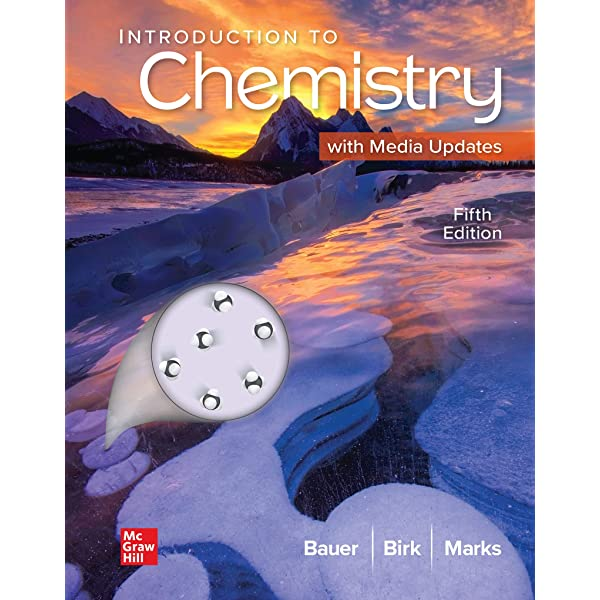
\includegraphics[scale=0.3]{bauer_text}
\end{center}

You may purchase your textbooks online from the Cypress College Online Bookstore
at \url{http://www.cypress.bkstr.com}

\begin{itemize}
\item \textbf{Lecture Textbook:} Bauer, R. C., Birk, J. P., and Marks, P. S., Introduction
  to Chemistry, McGraw Hill Companies, Inc., 5th Edition, 2019 ISBN- 9781260832303
  Discounted Edition (losse-leaf format) sold at Cypress College Bookstore 
  Hardcopy ISBN13: 9781259911149.
\item \textbf{Laboratory Textbook:} Hein, M., Custom Laboratory Manual Version A for CHEM107C,
  John Wiley \& Sons, 14th Edition ISBN-9781118975817.
  The eBook can also be purchased ISBN- 9781119784791, 1119784794.
  \url{https://www.vitalsource.com/custom/9781119784791}
  The custom manual contains excerpts from Foundations of Chemistry in the Laboratory
  (14th Edition) by Hein, Peisen, Best, and Miner.  Copyright: 2013 from John Wiley \& Sons,
  Inc. ISBN13: 9781118288993.
\item \textbf{Non-graphing, Non-programmable, Scientific Calculator:}
  A simple calculator with exponential, logarithmic, power, square roots functions in
  addition to its basic arithmetic capabilities. \textbf{Warning:} students will not be allowed
  to use any type of programmable calulators, phones, PDAs, and personal computers, etc.
  during quizzes and exams.
\item \textbf{Metric Ruler:} A simple metric ruler in the centimeter (cm) units with each individual
  line representing a millimeter (mm). 
\item \textbf{Crayons or Color Pencils:} A set of crayons or color pencils containing 12 basic colors.    
\end{itemize}

\section{Important Dates}
\begin{itemize}
\item The last day to add this class is September 5th.
\item The last day to drop this class without getting a “W” or a grade on your permanent
  record is September 5th.
\item Labor Day September 5th
\item Veteran’s Day November 11th
\item The last day to drop this class with a “W” on your permanent record is November 13th.
\item Thanksgiving Holiday November 24-25th
\item Final Exam in lecture classes Weds, December 7th 2:50 PM - 4:55 PM or
  Thursday, December 8th 1:45 PM - 3:50 PM (depending on the class you're enrolled in)
\end{itemize}

\section{Canvas Login Instructions}

This course will use Canvas as the “host”. Quizzes and assignments will be turned in
through Canvas. 

Canvas and is accessed through this web address: \url{http://cypresscollege.instructure.com}
NOTE: There is no “www” in the address. This web address is case and space sensitive. You should
bookmark this site (or put it in your favorites) for easy access. To login to the course site,
you must type in a “username” and “password.” Your username is your student ID number--including
the @ sign and all zeroes, for example, @00001234. Your password is the same one that you use
to register for classes. If you forgot your password, you may have to reset it.  

When you login to the Canvas website, the “dashboard” will open. There you will find the links
to your online course(s) which will appear as colored rectangular boxes. Click on the “CHEM 107C
Preparation for General Chemistry” course link and you will be taken to the course “Home” page. 

\subsection{Technical Requirements and Skills}
\begin{itemize}
\item Computer with a current operating system and a built-in or external camera and
  microphone
\item Current browser (Firefox or Chrome are preferable)
\item Stable internet connection
\item Basic internet skills (use of browser, searches, uploading/downloading files)
\item Scanning Device (a scanner or a tablet/smart phone with camera and scanner app).
\item Access to a printer is highly recommended
\end{itemize}

\section{Optional Classroom Health Measures}
\begin{itemize}
\item Wear a mask over your nose and mouth 
\item Practice social distancing from classmates and instructors whenever possible
\item Clean and disinfect your desk or lab station when you arrive
\end{itemize}

**Note health measures may change per CDC guidelines.

\section{Attendance Policy}

Attendance to lecture and laboratory is required for the entire designated time.
Any student who has more than three absences will be dropped from the class or
receive an F. For every three days of being late to class or leaving early, 10
points will be deducted from the student’s final grade, and will be counted as
the equivalent of one absence.


\section{Academic Honesty Policy}

All students should read the Academic Honesty Policy in the Cypress College catalog
and be certain that they fully understand it (see the instructor for further clarification
if necessary). Understanding the policy is essential, as academic dishonesty is a
serious offence that carries heavy penalties. Academic dishonesty may result in an
“F” on an assignment and referral to the dean.

\section{Academic Accommodations: Disability Support Services (DSS)}

Cypress College is committed to equitable access to educational opportunity.
Students with disabilities who may need an accommodation to fully participate in
this class should contact Disability Support Services (DSS) at 714.484.7104 or
dss-students@cypresscollege.edu.

If you have any other special needs for accessibility or any other issues,
(including, but not limited to, medical issues, physical/mental difficulties,
pregnancy), please discuss this with the instructor as soon as possible so that
appropriate accommodations can be made in timely manner. 

\section{Sexual Harassment/Discrimination Policy}

Students who believe they have been subjected to unlawful discrimination,
including sexual harassment, or who seek information regarding the District’s
Unlawful Discrimination Policy, should contact the Office of the District Director
of Human Resources at (714) 808-4818. 

\section{Message from SEM Counselors}

Do you have a comprehensive Student Educational Plan (SEP)? If not, please make
an appointment to speak with your academic counselor beginning the third week of
the semester. Counseling appointments are available from the third week through
the thirteenth week of each semester. 

\section{Grading Policy}

\begin{table}[H]
\label{tab:grade_policy}
\begin{tabular}{|l|p{0.72\linewidth}|l|}
  \hline
  \textbf{EXAMS} & Three exams will be given, each worth 125 points. Each exam
  will consist of a combination of multiple choice, short answer, and word problems.
  \textbf{If you cannot attend a scheduled exam, you must notify me before the day of the exam.
  Make-up exams must be taken within one week of the missed exam or zero credit will be
  given.}
  & $\mathbf{375}$ \\

  \textbf{QUIZZES} & 15 weekly quizzes worth 5 points each will be given over the course of
  the semester. Quizzes will include questions from lecture, lab, and assigned readings.
  Quizzes are assigned for each weekly module. Quizzes will consist of multiple choice,
  multiple answer, or fill in the blank. \textbf{Quizzes are given through Canvas and are due on
  Mons CRN 13199/Tues CRN 13196 at 11:59PM. You are only allowed to view one question at a
  time and given one attempt.}
  & $\mathbf{75}$ \\
  
  \textbf{HOMEWORK} & You will be expected to complete all assigned homework problems each week for
  10 points. Because exam questions will be based on homework problems, it is in your best
  interest to diligently complete all assignments. Be sure to write clearly, show calculations,
  and complete the problems in numerical order. \textbf{Homework will be due on Mons CRN 13199/
  Tues CRN 13196 at 11:59PM. Homework will be scanned and uploaded to Canvas as one pdf file.}
  & $\mathbf{150}$ \\

  \textbf{LABORATORY} & The lab will be graded on the quality and accuracy
    of your write-ups, and should reflect appropriate preparedness, technique, safety, and
    cleanliness for each lab assignment.
    \begin{itemize}
    \setlength\itemsep{0em}
    \item 15 Laboratory Reports and/or Handouts and Review
      (10 points each)
    \item Lab Practicum (50 points)
    \item Points will be deducted for leaving a messy lab drawer.
    \item Points will be deducted for not wearing goggles. Lab reports will be due
      on Mons CRN 13199/Tues CRN 13196  at 11:59PM.
    \item \textbf{Lab report pages as well as “Questions and Problems” from the lab
      manual will be scanned and uploaded to Canvas as one pdf file.}
    \item \textbf{Note: students must earn $70\%$ of the laboratory points to pass
      the course.}
    \end{itemize}
  & $\mathbf{200}$ \\

  \textbf{EXTRA CREDIT} & Extra credit may be given out. Keep a lookout for class announcements. & \\
    
  \textbf{FINAL EXAM} & A comprehensive final will be administered during finals week (200 points).
  & $\mathbf{200}$ \\

  \textbf{TOTAL} &  & $\mathbf{1000}$ \\
  \hline
\end{tabular}
\end{table}

\section{Chem 107C Calendar}

\begin{table}[H]
\label{tab:chem_cal}
\begin{tabular}{|p{0.15\linewidth}|p{0.35\linewidth}|p{0.35\linewidth}|p{0.1\linewidth}|}
  \hline
  & Lecture Chapter & Laboratory Experiment & Exams \\
  \hline
  \textbf{Week: 1 (8/22)} & Chapter 1 Math Toolbox & Math Tool Box Handouts &  \\
  
  \textbf{Week: 2 (8/29)} & Chapter 1 Matter and Energy & Lab Safety/Equipment Lab Safety Video and Quiz &  \\
  
  \textbf{Week: 3 M Holiday (9/5)} & Chapter 2 Atoms, Ions, and the Periodic Table & Laboratory Techniques
  \textbf{*Need the Lab Manual} &  \\

  \textbf{Week: 4 (9/12)} & Chapter 3 Chemical Compounds & Nomenclature (exercises 3, 4, 5) &  \\

  \textbf{Week: 5 M-holiday (9/19)} & Chapter 4 Chemical Composition & Measurements & Exam \#1 \\

  \textbf{Week: 6 (9/26)} & Chapters  4/5 Chemical Composition Chemical Reactions and Equations
  & Water in Hydrates &  \\

  \textbf{Week: 7 (10/3)} & Chapter 5 Chemical Reactions and Equations & Double Displacement Reactions &  \\

  \textbf{Week: 8 (10/10)} & Chapter 6 Quantities in Chemical Reactions & Single Displacement Reactions
  Electrolytes Demo (Part A) & \\

  \textbf{Week: 9 (10/17)} & Chapters 6/7 Quantities in Chemical Reactions Electron Structure of the Atom
  & Identification of Selected Anions & Exam \#2 \\

  \textbf{Week: 10 (10/24)} & Chapters 7/8 Electron Structure of the Atom Chemical Bonding
  & Quantitative Preparation of Potassium Chloride &  \\

  \textbf{Week: 11 (10/31)} & Chapter 8 Chemical Bonding & Electromagnetic Energy and Spectroscopy &  \\

  \textbf{Week: 12 (11/7)} & Chapter 9 The Gaseous State & Lewis Structures and Molecular Models &  \\

  \textbf{Week: 13 (11/14)} & Chapter 10 The Liquid and Solid States & Boyle’s Law & Exam \#3 \\

  \textbf{Week: 14 Th Holiday (11/21)} & Chapter 11 Solutions & Titrations &  \\

  \textbf{Week: 15 (11/28)} & Chapter 12/13 Reaction Rates and Chemical Equilibrium Acids and Bases
  & Lab Practicum &  \\

  \textbf{Week: 16 (12/5)} & Chapter 14/15 Oxidation-Reduction Reactions Nuclear Chemistry
  & Final Review & Final Exam  \\
  \hline
\end{tabular}
\end{table}

\section{Academic Honesty (From the Cypress College Catalog)}

Students are expected to abide by ethical standards in preparing and
presenting material which demonstrates their level of knowledge and which is
used to determine grades. Such standards are founded on basic concepts of
integrity and honesty. These include, but are not limited to the following areas:

\begin{enumerate}
\item Students shall not plagiarize, which is defined as stealing or passing
  off as one's own ideas or words of another and as using a creative production
  without crediting the source. The following cases are examples of what
  constitutes plagiarism:
  \begin{itemize}
  \item paraphrasing published material without acknowledging the source.
  \item  making significant use of an idea or a particular arrangement of ideas,
    e.g., outlines.
  \item  writing a paper after consulting with persons who provide suitable
    ideas and incorporating these ideas into the paper without acknowledging the debt.
  \item submitting under one’s own name, term papers or other reports which have
    been prepared by others.
  \end{itemize}
\item Students shall not cheat, which is defined as using notes, aids, or
  the help of other students on tests or exams in ways other than those expressly
  permitted by the instructor; and as misreporting or altering the data in laboratory
  or research projects involving the collection of data.
\item Students shall not submit an original paper or project to more than one class
  without approval from the second instructor. Instructors who do not accept previously
  submitted papers should so inform the students in the course syllabus.
\item Students shall not furnish materials or information in order to enable another
  student to plagiarize or cheat.
\end{enumerate}


An instructor who has evidence that an act of academic dishonesty has occurred,
after speaking with the student, is obligated to take the following steps:

\begin{enumerate}
\item Assign an appropriate academic penalty such as an oral reprimand (as in
  cases where there is reasonable doubt that the student knew that the action
  violated the standards of honesty); or assign an “F” on all or part of a particular
  paper, project, or exam (for example, where there was proof that it was a one-time
  occurrence). In cases where an “F” was assigned, report the incident to all
  appropriate personnel. (See Step 3).
\item In cases where the dishonesty was serious, premeditated, or part of an ongoing
  scheme, request an ad hoc review board made up of at least three faculty from the
  department or division of the instructor involved. This review board is to be
  appointed by the Academic Senate President or his/her delegate in consultation with
  the department coordinator, or if none is in place, with the members of the department.
  Supply to the review board the documents which are suspect and any other documents
  completed by the student which might help determine if academic dishonesty occurred.
  It would then be the responsibility of the review board to determine academic penalties
  as appropriate.
\item Report to the student involved, to the department coordinator, to the Division Dean,
  and to the Dean of Counseling and Student Development, the alleged incident of academic
  dishonesty, including relevant documentation, and recommendations for action that he
  or she deems appropriate.
\item The appropriate Division Dean shall maintain an academic dishonesty file of all cases
  of academic dishonesty with the appropriate documentation.
\item Students shall be informed when their names are inserted into the file and provided
  with copies of any appeals or disciplinary procedures in which they may become involved.
  The appropriate Division Dean may initiate disciplinary proceedings under Education Code,
  Article 3, Section 76030-76037; when two or more incidents involving the same student occur,
  he/she shall do so.
\item  Students charged with violations resulting in disciplinary action have the right
  to appeal the findings to the Petitions Committee under the Rules and Procedures of Due
  Process.
\end{enumerate}

\end{document}



